\documentclass{article}
\usepackage{amsmath, amssymb, ctex, graphicx, color}
\usepackage[margin=1in]{geometry}
\usepackage{setspace} % 行距控制
\usepackage{array}
\usepackage{makecell}
\usepackage{booktabs}

\usepackage{algorithm}
\usepackage{algpseudocode}
\usepackage{xcolor}
% 把默认注释符号 ▷ 改成行尾 // 等宽紫色，并右对齐
\renewcommand{\algorithmiccomment}[1]{\hfill\texttt{\textcolor{violet}{// #1}}}
% 定义 Input / Output 关键字（默认是 Require / Ensure）
\algnewcommand\algorithmicinput{\textbf{Input:}}
\algnewcommand\algorithmicoutput{\textbf{Output:}}
\algnewcommand\Input{\item[\algorithmicinput]}
\algnewcommand\Output{\item[\algorithmicoutput]}

\usepackage{titling}\setlength{\droptitle}{-2cm} 
\title{Ch9. REGULARIZATION \hfill 第9章 正则化 \\ 
Section 9.3. Learning Curves \hfill 第9.3节 学习曲线 \\ 
9.3.1 Early stopping \hfill 9.3.1. 早停法\\
9.3.2 Double descent \hfill 9.3.2. 双重下降}
\author{《深度学习基础》课程小组}
% \date{}
 
\begin{document}
\maketitle
% \tableofcontents

\setlength{\parindent}{0pt} % 取消首行缩进
\setlength{\parskip}{1.5em} % 设置段落之间的距离

\noindent\rule{\linewidth}{0.4pt}

\section{P1 Learning Curves}
We have already explored how the generalization performance of a model varies as we change the number of parameters in the model, the size of the data set, and the coefficient of a weight-decay regularization term. Each of these allows for a trade-off between bias and variance to minimize the generalization error. Another factor that influences this trade-off is the learning process itself. During optimization of the error function through gradient descent, the training error typically decreases as the model parameters are updated, whereas the error for hold-out data may be non-monotonic. This behaviour can be visualized using \emph{learning curves}, which plot performance measures such as training set and validation set error as a function of iteration number during an iterative learning process such as stochastic gradient descent. These curves provide insight into the progress of training and also offer a practical methodology for controlling the effective model complexity.

\noindent\rule{\linewidth}{0.4pt}

\section{P2 9.3.1 Early stopping}

An alternative to regularization as a way of controlling the effective complexity of a network is \emph{early stopping}. The training of deep learning models involves an iterative reduction of the error function defined with respect to a set of training data. Although the error function evaluated using the training set often shows a broadly monotonic decrease as a function of the iteration number, the error measured with respect to hold-out data, generally called a validation set, often shows a decrease at first, followed by an increase as the network starts to over-fit. To obtain a network with good generalization performance, training should be stopped at the point of smallest error with respect to the validation data set, as indicated in Figure~9.7.

Figure 9.7 Caption: An illustration of the behaviour of training set error (left) and validation set error (right) during a typical training session, as a function of the iteration step, for the sinusoidal data set. To achieve the best generalization performance, the training should be stopped at the point shown by the vertical dashed lines, corresponding to the minimum of the validation set error.

\begin{figure}[htbp]
    \centering
    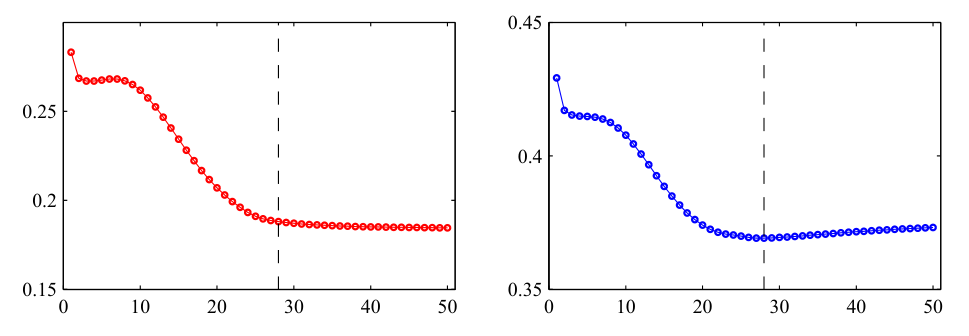
\includegraphics[width=0.5\textwidth]{figure-9-7.png}
    \caption{图9-7：训练误差和验证误差}
    % \label{}
\end{figure}

\noindent\rule{\linewidth}{0.4pt}

\section{P3}

This behaviour of the learning curves is sometimes explained qualitatively in terms of the effective number of parameters in the network. This number starts out small and then grows during training, corresponding to a steady increase in the effective complexity of the model. Stopping training before a minimum of the training error has been reached is a way to limit the effective model complexity.

\noindent\rule{\linewidth}{0.4pt}

\section{P4}

We can verify this insight for a quadratic error function and show that early stopping should exhibit similar behaviour to regularization using a simple weight-decay term (Bishop, 1995a). This can be understood from Figure~9.8, in which the axes in weight space have been rotated to be parallel to the eigenvectors of the Hessian matrix. If, in the absence of weight decay, the weight vector starts at the origin and proceeds during training along a path that follows the local negative gradient vector, then the weight vector will move initially parallel to the $w_2$ axis through a point corresponding roughly to $\bar{\mathbf{w}}$ and then move towards the minimum of the error function $\mathbf{w}_{\text{ML}}$. This follows from the shape of the error surface and the widely differing eigenvalues of the Hessian. Stopping at a point near $\bar{\mathbf{w}}$ is therefore similar to weight decay, thereby showing that the quantity $\tau/\eta$ (where $\tau$ is the iteration index and $\eta$ is the learning rate parameter) acts like the reciprocal of the regularization parameter $\lambda$. The effective number of parameters in the network therefore grows during training.

Figure 9.8 Caption: A schematic illustration of why early stopping can give similar results to weight decay for a quadratic error function. The ellipses show contours of constant error, and $\mathbf{w}^*$ denotes the maximum likelihood solution corresponding to the minimum of the unregularized error function. If the weight vector starts at the origin and moves according to the local negative gradient direction, then it will follow the path shown by the curve. By stopping training early, a weight vector $\bar{\mathbf{w}}$ is found that is qualitatively like that obtained with a simple weight-decay regularizer along with training to the minimum of the regularized error, as can be seen by comparing with Figure 9.3.

\begin{figure}[htbp]
    \centering
    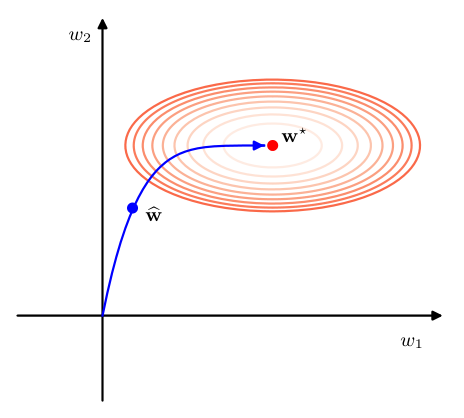
\includegraphics[width=0.5\textwidth]{figure-9-8.png}
    \caption{图9-8：早停法的效果}
    % \label{}
\end{figure}

\noindent\rule{\linewidth}{0.4pt}

\section{P5 9.3.2 Double descent}

The bias--variance trade-off provides insight into the generalization performance of a learnable model as the number of parameters is varied. Models with too few parameters will have a high test set error due to the limited representational capacity (high bias), and as the number of parameters increases, the test error is expected to fall. However, as the number of parameters is increased further, the test error increases again due to over-fitting (high variance). This leads to the conventional belief, widespread in classical statistics, that the number of parameters in the model needs to be limited according to the size of the data set and that for a given training data set, very large models are expected to have poor performance.

\noindent\rule{\linewidth}{0.4pt}

\section{P6}

Contrary to this expectation, however, modern deep neural networks can have excellent performance even when the number of parameters far exceeds that required to achieve a perfect fit to the training data (Zhang et al., 2016), and the general wisdom in the deep learning community is that bigger models are better. Although early stopping is sometimes used, models may also be trained to zero error and yet still have good performance on test data.

\noindent\rule{\linewidth}{0.4pt}

\section{P7}

This seemingly contradictory perspective can be reconciled by examining learning curves and other plots of generalization performance versus model complexity, which reveal a more subtle phenomenon called \emph{double descent} (Belkin et al., 2019). This is illustrated in Figure~9.9, which shows training set and test set errors versus model complexity, as determined by the number of learnable parameters, for a large neural network called ResNet18 (He et al., 2015a), which has 18 layers of parameters trained on an image classification task. The number of weights and biases in the network is varied by changing the `width parameter', which governs the number of hidden units in each layer. We see that the training error decreases monotonically with increasing complexity of the model, as expected. However, the test set error decreases at first then increases again and then finally decreases again. This reduction in test set error for very large models continues even after the training set error has reached zero.

Figure 9.9 Caption: Plot of training set and test set errors for a large neural network model called ResNet18 trained on an image classification problem versus the complexity of a model. The horizontal axis represents a hyperparameter governing the number of hidden units and hence the overall number of weights and biases in the network. The vertical dashed line, labelled `interpolation threshold' indicates the level of model complexity at which the model is capable, in principle, of achieving zero error on the training set. [From Nakkiran et al.\ (2019) with permission.]

\begin{figure}[htbp]
    \centering
    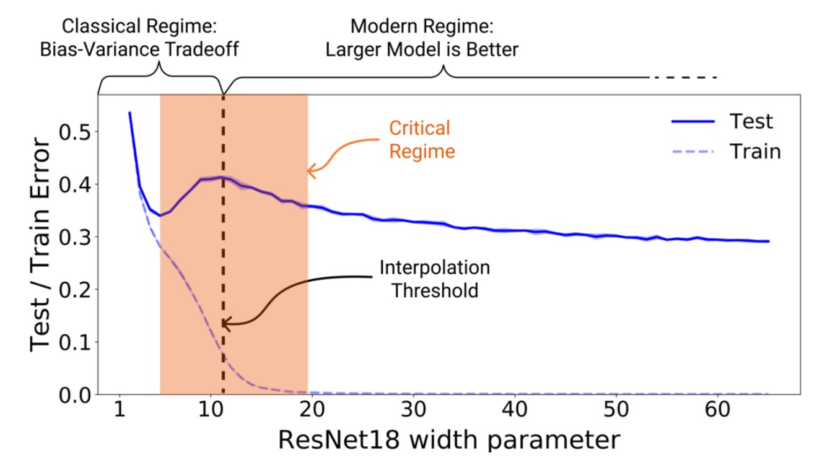
\includegraphics[width=0.5\textwidth]{figure-9-9.png}
    \caption{图9-9：ResNet18的训练误差与测试误差}
    % \label{}
\end{figure}

\noindent\rule{\linewidth}{0.4pt}

\section{P8}

This surprising behaviour is more complex than we would expect from the usual bias--variance discussion of classical statistics and exhibits two different regimes of model fitting, as shown schematically in Figure~9.9, corresponding to the classical bias--variance trade-off for small to medium complexity, followed by a further reduction in test set error as we enter a regime of very large models. The transition between the two regimes occurs roughly when the number of parameters in the model is sufficiently large that the model is able to fit the training data exactly (Belkin et al., 2019). Nakkiran et al.\ (2019) define the \emph{effective model complexity} to be the maximum size of training data set on which a model can achieve zero training error, and so double descent arises when the effective model complexity exceeds the number of data points in the training set.

\noindent\rule{\linewidth}{0.4pt}

\section{P9}

We see similar behaviour if we control model complexity using early stopping, as seen in Figure~9.10. Increasing the number of training epochs increases the effective model complexity, and for a sufficiently large model, double descent is again observed. For such models there are many possible solutions including those that over-fit to the data. It therefore seems to be a property of stochastic gradient descent that the implicit biases that it introduces lead to good generalization performance.

Figure 9.10 Caption: Plot of test set error versus number of epochs of gradient descent training for ResNet18 models of various sizes. The effective model complexity increases with the number of training epochs, and the double descent phenomenon is observed for a sufficiently large model. [From Nakkiran et al.\ (2019) with permission.]

\begin{figure}[htbp]
    \centering
    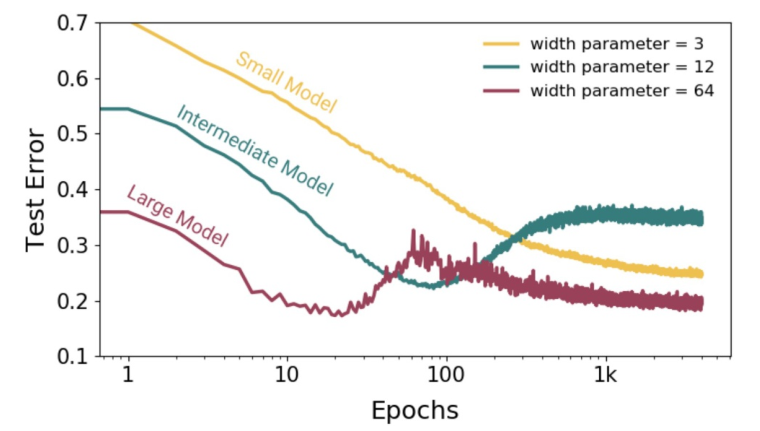
\includegraphics[width=0.5\textwidth]{figure-9-10.png}
    \caption{图9-10：ResNet18的测试误差与训练次数}
    % \label{}
\end{figure}

\noindent\rule{\linewidth}{0.4pt}

\section{P10}

Analogous results are also obtained when a regularization term in the error function is used to control complexity. Here the test set error of a large model trained to convergence shows double descent with respect to $1/\lambda$, the inverse regularization parameter, since high $\lambda$ corresponds to low complexity (Yilmaz and Heckel, 2022).

\noindent\rule{\linewidth}{0.4pt}

\section{P11}

One ironic consequence of double descent is that it is possible to operate in a regime where increasing the size of the training data set could actually reduce performance, contrary to the conventional view that more data is always a good thing. For a model in the critical regime shown in Figure~9.9, an increase in the size of the training set can push the interpolation threshold to the right, leading to a higher test set error. This is confirmed in Figure~9.11, which shows the test set error for a transformer model as a function of the dimensionality of the input space, known as the embedding dimension. Increasing the embedding dimension increases the number of weights and biases in the model and hence increases the model complexity. We see that increasing the training set size from 4,000 to 18,000 data points leads to a curve that is overall much lower. However, for a range of embedding dimensions that correspond to models in the critical complexity regime, increasing the size of the data set can actually reduce generalization performance.

Figure 9.11 Caption: Plot of test set error for a large transformer model versus the embedding dimension, which controls the number of parameters in the model. Increasing the size of the training set from 4,000 to 18,000 samples generally leads to a lower test set error, but for some intermediate values of model complexity, there can be an increase in the error, as shown by the vertical red arrows. [From Nakkiran et al. (2019) with permission.]

\begin{figure}[htbp]
    \centering
    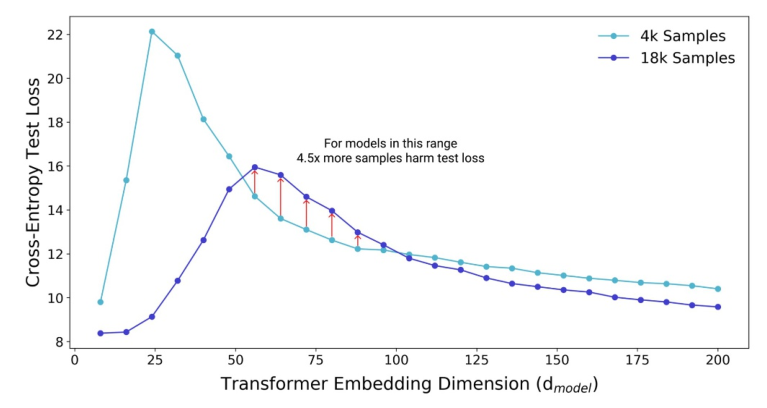
\includegraphics[width=0.5\textwidth]{figure-9-11.png}
    \caption{图9-11：Transformer模型的测试误差}
    % \label{}
\end{figure}

\end{document}

